\capa

% \pretextualchapter{}

\folhaderosto
% 
\pretextualchapter{}
	\thispagestyle{plain}
	\noindent \parbox{5.7in}{\centering AUTORIZO A REPRODUÇÃO E DIVULGAÇÃO TOTAL OU PARCIAL DESTE TRABALHO, POR QUALQUER MEIO CONVENCIONAL OU ELETRÔNICO, PARA FINS DE ESTUDO E PESQUISA, DESDE QUE CITADA A FONTE.}

\pretextualchapter{}



%\afterpage{\blankpage}
%
%\pretextualchapter{DEDICATÓRIA} %Título da página dedicatória
%	\input{dedicatoria} %Para incluir o texto de dedicatória,use o arquivo dedicatória.tex

\afterpage{\blankpage}


\pretextualchapter{AGRADECIMENTOS} %Título da página de agradecimentos
	
Sinceros agradecimentos ao Prof. Gonzalo Travieso e ao Prof. Luciano da Fontoura
Costa. Tenham certeza que foi com vocês que aprendi o que é fazer
pesquisa. Foram ensinamentos que guardarei para toda a vida. Além da orientação
de excelência, ficará para sempre a amizade.

\vspace{4 mm}

Aos meus queridos pais, Vilson e Salete, sabem que devo tudo o que sou a
vocês. Encontro sempre suas palavras de conforto e sabedoria em cada esquina que
cruzo, em cada caminho que percorro. Amo muito vocês.

\vspace{4 mm}

À minha amada, Gabriela, que esteve ao meu lado em cada momento, bom ou ruim,
por seu amparo, carinho e cumplicidade. Te amo.

\vspace{4 mm}

À Paulo e Lourdes pelas conversas sempre animadas, e à Isabela pelas
risadas sempre prontas às minhas piadas :-D

\vspace{4 mm}

Aos meus irmãos Renato e Ricardo Fabbri, que me acolhem com tanto carinho e com
quem espero viver ainda ótimas passagens. Renato, obrigado por ser um verdadeiro
mentor.

\vspace{4 mm}

Ao bom amigo e conselheiro Pedro Kroeger, continuas sendo a quem sigo os passos.

\vspace{4 mm}

A todos do labMacambira.sf.net, por todas as colaborações e aprendizados, seja
artisticamente, cientificamente, socialmente, em \emph{software},
em \emph{tinta}, em \emph{notas} ou em \emph{espírito}.

\vspace{4 mm}

À Mozilla Foundation e seus colaboradores, em especial ao bom amigo Forrest
Oliphant, que me mentorou enquanto participante do Googler Summer of Code 2012 e
com quem continuo compartilhando ótimas conversas e desenvolvimentos. Thank you Fo!

\vspace{4 mm}

A todos os amigos que fiz no IFSC/USP, em especial Carlos Doro Neto (valeu
pelo \textit{Doro's method}!), David Sbrissa (\textit{bit******!}),
prof. Osvaldo ``Chu'', prof. Rodrigo Guido, profa. Yvonne Mascarenhas, Débora
Correa, Mauro Miazaki, Diego, César, Thomás, Filipi. Aos parceiros
do \textit{hacklab do velho}, tenho grande carinho por todos vocês.

\vspace{4 mm}

Não sei se conseguirei lembrar de todos, mas meu especial agradecimento e grande
carinho a Daniel Penalva, Caleb Luporini, Guilherme Lunhani, Geraldo Magela
Rocha, Glerm Soares, Chico e Fábio Simões, Daniel Marostegan, prof. Rogério
``Zeco'' Silva, Gilson Beck, Marcos Mendonça, Danilo Shiga, Edson Corrêa,
Vanessa Ferreira, prof. Luis Castelões, Luis Fernando Muniz Cirne, Marília
Pisani, prof. Massimo Canevacci. À Teia Casa de Criação e Pontão Nós Digitais,
ao MuSA, aos amigos da Udesc, à galera do AVAV, do Crânio Sonante, a todos que
tive contato real e virtualmente, nas listas de email, AA, IRC e outras redes e
canais.

\vspace{4 mm}

Agradeço às comunidades de cultura e software livre e aberto por todos os
conhecimentos e tecnologias repassados e que compõem esta contribuição.

\vspace{4 mm}

\begin{center}
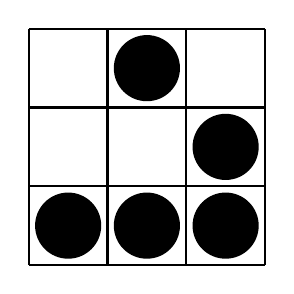
\begin{tikzpicture}[thick]
\draw (0,0) grid (3,3);
\foreach \c in {(0,0), (1,0), (2,0), (2,1), (1,2)}
    \fill \c + (0.5,0.5) circle (0.42);
\end{tikzpicture}
\end{center}
 %Para incluir o texto de agradecimentos,use o arquivo agradecimentos.tex


\pretextualchapter{}
	\begin{epigrafetop}
		{A arte é feita para perturbar. A ciência tranquiliza. Na arte só uma coisa importa: aquilo que não se pode explicar.}
        {Goerges Braque}
	\end{epigrafetop}

	\begin{epigrafemid}
		{A ciência é tudo aquilo que conseguimos explicar a um computador. Todo o resto é arte.}
		{Donald Knuth}
	\end{epigrafemid}
	\vspace{-1cm}

	\begin{epigrafebot}
                {Todos querem entender de arte. Por que não tentam entender o
                canto de um pássaro?}
                {Pablo Picasso}
	\end{epigrafebot}



\afterpage{\blankpage}

\resumoeabstract %Para incluir o texto do resumo e abstract,use o arquivo resumoeabstract.tex

\afterpage{\blankpage}


\listadefiguras %Comando que gera a lista de figuras (AUTOMÁTICO)

%\listadetabelas %Comando que gera a lista de tabelas (AUTOMÁTICO)

\afterpage{\blankpage}
%% \pretextualchapter{LISTA DE RELAÇÕES ANALÍTICAS DESCRITAS E IMPLEMENTADAS COMPUTACIONALMENTE NO APÊNDICE~\ref{cap:codigoProc}}
%% 	\begin{listaespecial}[BIGNAMEWIDTH]
%%         \item[Equação~\ref{eq:dur}] Sequência de amostras de um áudio PCM.
%%         \item[Equação~\ref{eq:potencia}] Potência.
%%         \item[Equação~\ref{decibels}] Decibels entre dois áudios.
%%         \item[Equação~\ref{eq:ampVol}]  Amplitude dobrada em decibels.
%%         \item[Equação~\ref{eq:potVol}] Potência dobrada em decibels.
%%         \item[Equação~\ref{eq:dobraVol}] Variação de amplitude no volume dobrado (10 dBs).
%%         \item[Equação~\ref{ampDec}] Conversão de decibels em variação de amplitude.
%%         \item[Equação~\ref{periodicidade}] Representação básica de uma sequência periódica.
%%         \item[Equação~\ref{senoide}] Sequência infinita senoidal.
%%         \item[Equação~\ref{denteDeSerra}] Sequência infinita de uma onda 'dente de serra'.
%%         \item[Equação~\ref{triangular}] Sequência infinita de uma onda 'triangular'.
%%         \item[Equação~\ref{quadrada}] Sequência infinita de uma onda 'quadrada'.
%%         \item[Equação~\ref{sampleandoFormaDeOnda}] Sequência infinita de uma forma de onda \emph{sampleada}.
%%         \item[Equação~\ref{recomposicaoFourier}] Recomposição das amostras temporais com base nos coeficientes espectrais.
%%         \item[Equação~\ref{moduloEfase}] Recomposição das amostras temporais reais em termos do módulo e fase.
%%         \item[Equação~\ref{coefsPareados}] Número de pares de coeficientes relativos à mesma frequência.
%%         \item[Equação~\ref{equivalenciasFreqs}] Coeficientes equivalentes em termos das frequêcias que representam.
%%         \item[Equação~\ref{equivalenciasModulos}] Equivalências dos módulos dos coeficientes espectrais.
%%         \item[Equação~\ref{equivalenciasFases}] Equivalências das fases dos coeficientes espectrais.
%%         \item[Equação~\ref{eq:reconsCompleta}] Reconstrução das amostras temporais em termos dos coeficientes pareados e independentes.
%%         \item[Equação~\ref{eq:notaBasica}] Nota básica com duração, frequência e altura.
%%         \item[Equação~\ref{periodoUnico}] Forma de onda sintética ou amostrada.
%%         \item[Equação~\ref{eq:notaBasicaTimbre}] Nota básica com forma de onda especificada.
%%         \item[Equação~\ref{eq:distOuvidos}] Distância de uma fonte sonora a cada ouvido.
%%         \item[Equação~\ref{eq:dti}] Diferença de Tempo Interaural (DTI).
%%         \item[Equação~\ref{eq:dii}] Diferença de Intensidade Interaural (DII).
%%         \item[Equação~\ref{eq:locImpl}] Sequência binaural PCM com  DTI e DII para localização espacial.
%%         \item[Equação~\ref{eq:angulo}] Ângulo resolvido pela implementação da DTI e DII.
%%         \item[Equação~\ref{eq:mixagem}] Mixagem de N sequências.
%%         \item[Equação~\ref{eq:concatenacao}] Concatenação de N sequências.
%%         \item[Equação~\ref{eq:lut}] Procedimento de busca em tabelas (\emph{Lookup Table}).
%%         \item[Equação~\ref{freqLinear}] Frequências em cada amostra em uma variação linear.
%%         \item[Equação~\ref{indiceLinear}] Índices para busca na tabela em uma variação linear de frequência.
%%         \item[Equação~\ref{serieAmostralLin}] Sequência amostral em uma variação linear de frequências.
%%         \item[Equação~\ref{freqExponencial}] Frequências em cada amostra em uma variação exponencial.
%%         \item[Equação~\ref{indiceExponencial}] Índices para busca na tabela em uma variação exponencial de frequência.
%%         \item[Equação~\ref{serieAmostralLog}] Sequência amostral em uma variação exponencial de frequências.
%%         \item[Equação~\ref{seqAmp}] Sequência de amplitudes em uma variação exponencial.
%%         \item[Equação~\ref{transAmp}] Sequência amostral em uma variação exponencial de amplitude.
%%         \item[Equação~\ref{seqAmpLin}] Sequência de amplitudes em uma variação linear de amplitude.
%%         \item[Equação~\ref{seqAmpDB}] Sequência amostral em uma variação exponencial de amplitude dada em decibels.
%%         \item[Equação~\ref{eq:conv}] Convolução de sequências reais e finitas.
%%         \item[Equação~\ref{eq:diferencas}] Equação a diferenças para aplicação temporal de filtros IIR.
%%         \item[Equação~\ref{eq:passa-baixas}] Coeficientes de um filtro passa-baixas bem comportado de primeira ordem com frequência de corte variável.
%%         \item[Equação~\ref{eq:passa-altas}] Coeficientes de um filtro passa-altas bem comportado de primeira ordem com frequência de corte variável.
%%         \item[Equação~\ref{eq:varAux}] Variáveis auxiliares de um filtro nó de segunda ordem.
%%         \item[Equação~\ref{eq:passa-banda}] Coeficientes de um filtro passa-banda de segunda ordem com frequência central e largura de banda variáveis.
%%         \item[Equação~\ref{eq:rejeita-banda}] Coeficientes de um filtro rejeita-banda de segunda ordem com frequência central e largura de banda variáveis.
%%         \item[Equação~\ref{eq:branco}] Coeficientes espectrais para síntese de ruído branco.
%%         \item[Equação~\ref{eq:rosa}] Coeficientes espectrais para síntese de ruído rosa.
%%         \item[Equação~\ref{eq:marrom}] Coeficientes espectrais para síntese de ruído marrom.
%%         \item[Equação~\ref{eq:azul}] Coeficientes espectrais para síntese de ruído azul.
%%         \item[Equação~\ref{eq:violeta}] Coeficientes espectrais para síntese de ruído violeta.
%%         \item[Equação~\ref{eq:preto}] Coeficientes espectrais para síntese de ruído preto.
%%         \item[Equação~\ref{vbrGamma}] Índices auxiliares para um vibrato de frequência variável.
%%         \item[Equação~\ref{vbrAux}] Expoentes auxiliares para um vibrato de frequência variável.
%%         \item[Equação~\ref{vbrF}] Frequências por amostra de um vibrato de frequência e profundidade variáveis.
%%         \item[Equação~\ref{vbrGamma2}] Índices um vibrato de frequência e profundidade variáveis.
%%         \item[Equação~\ref{vbrT}] Amostras de um áudio com vibrato de frequência e profundidade variáveis.
%%         \item[Equação~\ref{trA}] Amplitudes por amostra de um tremolo de frequência e profundidade variáveis.
%%         \item[Equação~\ref{trT}] Amostras de um áudio com tremolo de frequência e profundidade variáveis.
%%         \item[Equação~\ref{eq:fmEsp}] Espectro da síntese FM.
%%         \item[Equação~\ref{eq:amEsp}] Espectro da síntese AM.
%%         \item[Equação~\ref{fmGammaAux}] Índices auxiliares para síntese FM.
%%         \item[Equação~\ref{fmAux}] Sequência auxiliar para síntese FM.
%%         \item[Equação~\ref{fmF}] Sequência de frequências para cada amostra para síntese FM.
%%         \item[Equação~\ref{fmGamma}] Índices para síntese FM.
%%         \item[Equação~\ref{fmT}] Sequência amostral resultante da síntese FM.
%%         \item[Equação~\ref{amA}] Sequência de amplitudes por amostra na síntese AM.
%%         \item[Equação~\ref{amT}] Sequência amostral resultante da síntese AM.
%%         \item[Equação~\ref{eq:vinculos}] Exemplo de vínculo entre a frequência e parâmetros do tremolo e do vibrato em um som.
%%         \item[Equação~\ref{eq:fDoppler}] Equação básica da frequência observada no efeito Doppler.
%%         \item[Equação~\ref{eq:aDoppler}] Amplitude observada no efeito Doppler.
%%         \item[Equação~\ref{eq:ffDoppler}] Frequência efetiva observada no efeito Doppler.
%%         \item[Equação~\ref{eq:p1rev}] Primeiro período de uma reverberação.
%%         \item[Equação~\ref{eq:p2rev}] Segundo período de uma reverberação.
%%         \item[Equação~\ref{eq:rev}] Resposta ao impulso de uma reverberação.
%%         \item[Equação~\ref{eq:adsr}] Envoltória ADSR com variações lineares e logarítmicas.
%%         \item[Equação~\ref{eq:adsrApl}] Aplicação da envoltória ADSR em uma sequência arbitrária.
%%         \item[Equação~\ref{eq:intervalos}] Intervalos musicais em número de semitons.
%%         \item[Equação~\ref{escSim}] Escalas simétricas na oitava divida em 12 notas.
%%         \item[Equação~\ref{eq:escalas}] Escalas diatônicas.
%%         \item[Equação~\ref{eq:relacaoDia}] Sucessão de intervalos em uma escala diatônica.
%%         \item[Equação~\ref{eq:escalasMenores}] Escalas menores natural, harmônica e melódica.
%%         \item[Equação~\ref{triades}] Tríades maior, menor, diminuta e aumentada.
%%         \item[Subseção~\ref{subsec:intervalos}] Relações microtonais através de frações de semitons ou através de quantidades inteiras de divisões arbitrárias da oitava.
%%         \item[Subseção~\ref{subsec:harmonia}] Relações básicas de harmonia tonal.
%%         \item[Subseção~\ref{subsec:contraponto}] Regras básicas de condução de vozes com independência.
%%         \item[Subseção~\ref{subsec:ritmo}] Relações básicas de métrica e rítmica.
%%         \item[Subseção~\ref{subsec:dir}] Formação de arcos musicais através de estruturas direcionais.
%%         \item[Subseção~\ref{estCic}] Estruturas cíclicas para a síntese musical.
%% %        \item[Equação~\ref{eq:groups}] Propriedades básicas de um grupo algébrico.

%% 	\end{listaespecial} 


%% \pretextualchapter{Elementos de notação}
%% 	\begin{listaespecial2}[BIGNAMEWIDTH]
%%         \item[$Hz$] abreviação de Herz, medida de frequência, número de ocorrências por segundo.
%%         \item[$kHz$] abreviação de kilo Hertz, i.e. mil Herz.
%%         \item[$m$] metro.
%%         \item[$mm$] milímetro.
%%         \item[$s$] segundo.
%%         \item[$m/s$] metros por segundo.
%%         \item[$f_a$] frequência de amostragem, taxa de amostragem.
%%         \item[$\lambda_a$] duração da separação temporal entre um par de amostras consecutivas.
%%         \item[PCM] sigla de \emph{Pulse Code Modulation}, veja seção~\ref{sec:audio}
%%         \item[$S_i$] sequência $S$ indexada em $i$.
%%         \item[$\{s_i\}_x^{y}$] sequência com elementos $s_i$ com índices de $x$ a $y$ incluso.
%%         \item[$\lfloor x \rfloor$] parte inteira de $x$.
%%         \item[$V_{dB}$] volume em decibels.
%%         \item[$\Rightarrow$] então.
%%         \item[$\therefore$] portanto.
%%         \item[$:$] tal que.
%%         \item[$\forall$] para todo.
%%         \item[$\approx$] aproximadamente.
%%         \item[$\equiv$] equivalente.
%%         \item[$\%$] operação módulo, resto da divisão.
%%         \item[$\Lambda$] comprimento em amostras.
%%         \item[$\widetilde{\Lambda}$] comprimento em amostras de período de onda.
%%         \item[$\Delta$] duração temporal.
%%         \item[$a_i$] fator multiplicativo de amplitude da $i$-ésima amostra.
%% 	\end{listaespecial2} 


%
%\afterpage{\blankpage}
%
%\pretextualchapter{Lista de peças musicais}
%	\begin{listaespecial}[BIGNAMEWIDTH]
%		\item[Chorus infantil]: relações harmônicas da seção~\ref{}. Música disponibilizada online~\cite{}. Arquivo Python no apêndice~\ref{}.
%	\end{listaespecial} 
%
%\afterpage{\blankpage}
%\pretextualchapter{Lista de Abreviaturas}
%	\begin{listaespecial}[BIGNAMEWIDTH]
%		\item[OSS] Programas de Código Aberto \emph{(Open Source Software)}
%		\item[GNU] \emph{GNU is Not UNIX}
%		\item[GPL] \emph{General Public Licence}
%                \item[AA] \emph{Algorithmic Autoregularion ou Acrônimo Ambíguo}
%                \item[AC] \emph{Autogestão Coletiva ou Ágora Communs}
%                \item[CC] \emph{Creative Commons}
%                \item[ABT] \emph{ABeatTracker}
%                \item[ABD] \emph{ABeatDetector}
%                \item[PD] \emph{Pure Data}
%                \item[CMDCA] \emph{Conselho Municipal de defesa dos Direitos da Cirança e do Adolescente}
%                \item[SOS] \emph{Saúde Olha Sabedoria: uma proposta de coleta e difusão de conhecimentos relacionados à saúde}
%                \item[LADSPA] \emph{Linux Audio Developers Simple Plugin API}
%                \item[LV2] \emph{LADSPA Version 2}
%                \item[JACK] \emph{Jack Audio Connection Kit}
%                \item[SIP] \emph{Scilab Imaging Processing toolbox}
%                \item[MIT] \emph{Massachusetts Institute of Technology}
%                \item[NUMPY] \emph{Numerical Python}
%                \item[SCIPY] \emph{Scientific Python}
%                \item[ONU] \emph{Organização das Nações Unidas}
%                \item[SL] \emph{Software Livre}
%                \item[EKP] \emph{Emotional Kernel Panic}
%                \item[SOS] \emph{Saúde Olha Sabedoria}
%                \item[FISL] \emph{Festival Internacional de Software Livre}
%                \item[BPM] \emph{Batidas Por Minuto (medida de andamento musical)}
%                \item[API] \emph{Application Programming Interface ou Interface de Programação de Aplicativos}
%                \item[WP] \emph{Wavelet Packet}
%
%		\item[EL] \emph{Estúdio Livre}
%		\item[AE] \emph{AudioExperiments}
%		\item[PCM] \emph{Pulse Code Modulation (modulação por código de pulsos)}
%		\item[DTI] \emph{Diferença de Tempo Interaural (\emph{Interaural Time Difference} - ITD)}
%		\item[DII] \emph{Diferença de Intensidade Interaural (\emph{Interaural Intensity Difference)} - IID ou \emph{Interaural Level Difference} - ILD}
%	\end{listaespecial} 
%

\sumario

